\documentclass[12pt]{article}
\usepackage[utf8]{inputenc}
\usepackage{amsfonts}
\usepackage{graphicx}
\usepackage{caption}
\usepackage{subcaption}
\usepackage{amssymb}
\usepackage{tikz}
\usepackage{tabularx}
\usepackage{listings}
\usepackage{xcolor}
\usepackage{xlop}
\usepackage{supertabular}
\usepackage{multicol}

\definecolor{codegreen}{rgb}{0,0.6,0}
\definecolor{codegray}{rgb}{0.5,0.5,0.5}
\definecolor{codepurple}{rgb}{0.58,0,0.82}

\newcommand{\n}{\vspace{2.5mm} \newline}
\renewcommand{\figurename}{Figura}

\title{Càlcul de fractals en paral·lel}
\author{Àlex Palomas Jiménez}
\date{2021-2022}

\begin{document}
\pagenumbering{gobble}
\maketitle
\newpage

\renewcommand\contentsname{Índex:}
\tableofcontents
\newpage
\pagenumbering{arabic}


\section{Introducció}

\subsection{La fractal}
Una fractal és una figura, que pot ser espacial o plana, formada per components infinits. És a dir, si ens apropem veurem que no té fi. La seva principal característica és l'autosimilitud, exacta o no. Per exemple, en la figura \ref{fig:sierpinski}, podem veure el triangle de Sierpinski. Aquest té una autosimilitud exacta, doncs si ens apropem ens trobem amb la mateixa figura. En canvi, en la figura \ref{fig:mandelbrot}, el conjunt de Mandelbrot, no es autosimilar exacte, doncs si ens anem apropant ens surt la mateixa figura pero de vegades girada i això provoca que no sigui exacte.

\begin{figure}[h]
    \centering
    \begin{minipage}{.5\textwidth}
      \centering
      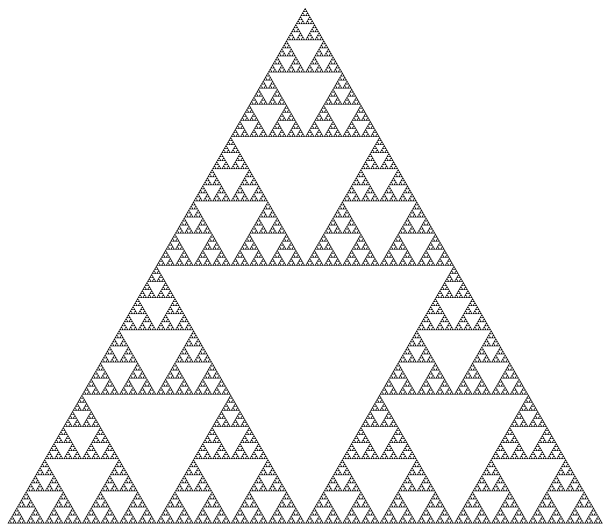
\includegraphics[width=.8\linewidth]{imatges/sierpinski.jpg}
      \captionof{figure}{Triangle de Sierpinski.}
      \label{fig:sierpinski}
    \end{minipage}%
    \begin{minipage}{.5\textwidth}
      \centering
      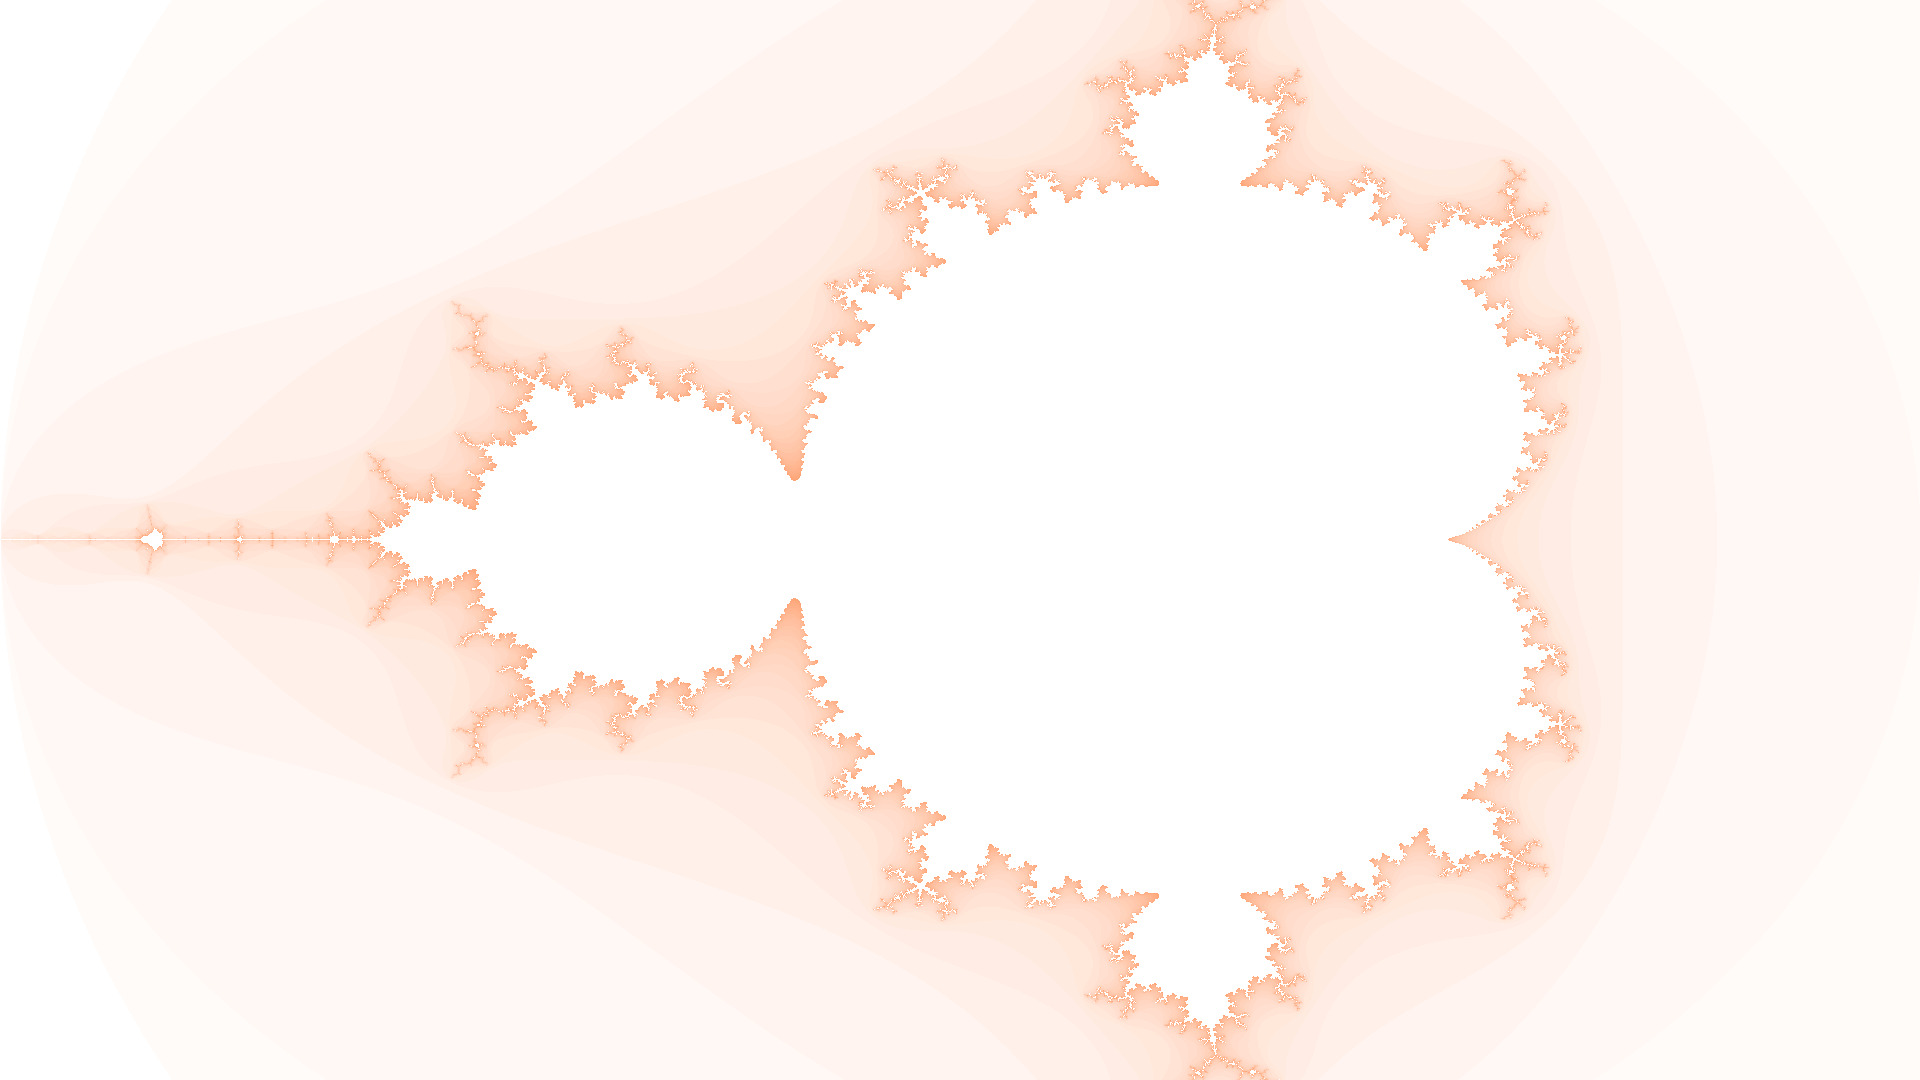
\includegraphics[width=.8\linewidth]{imatges/Captured_On_Mon_Dec__6_18-48-29_2021-.jpg}
      \captionof{figure}{Conjunt de Mandelbrot}
      \label{fig:mandelbrot}
    \end{minipage}
\end{figure}


\noindent Una característica que tenen tots els fractals és la seva dimensió. Aquesta moltes vegades es, fins i tot irracional. No sol ser 1 ni 2 ni 3. Per exemple, el triangle en la figura \ref{fig:sierpinski} és de dimensió $\frac{ln 3}{ln 2} \approx 1,585$. En canvi la dimensió del parímetre del conjunt de Mandelbrot, en la figura \ref{fig:mandelbrot} és de: 2. \n

\noindent Hi ha molts tipus de fractals, aquests son utilitzats desde els camps de l'art fins els camps de computació amb la compressió d'imatges i nombres pseudoaleatoris fins a la neurociència. També s'utilitzen per estudiar la formació de les estrelles, doncs els núbols de partícules es formen a partir del principi d'autosimilitud. Es pot estudiar fins i tot l'evolució del canvi climàtic. Doncs les fractals, en alguns casos, son sistemes caòtics.


\subsection{Nombres complexos}
Dins dels nombres existeixen per ordre: els nombres naturals ($\mathbb{N}$), els quals es troben dins dels enters ($\mathbb{Z}$), els quals formen part dels nombres racionals ($\mathbb{Q}$) i aquests, juntaments amb els irracionals formen part dels nombres reals ($\mathbb{R}$). Aquests amb els nombres imaginaris ($\mathbb{I}$) formen part dels complexos, representats amb el símbol $\mathbb{C}$.\n
\centerline {
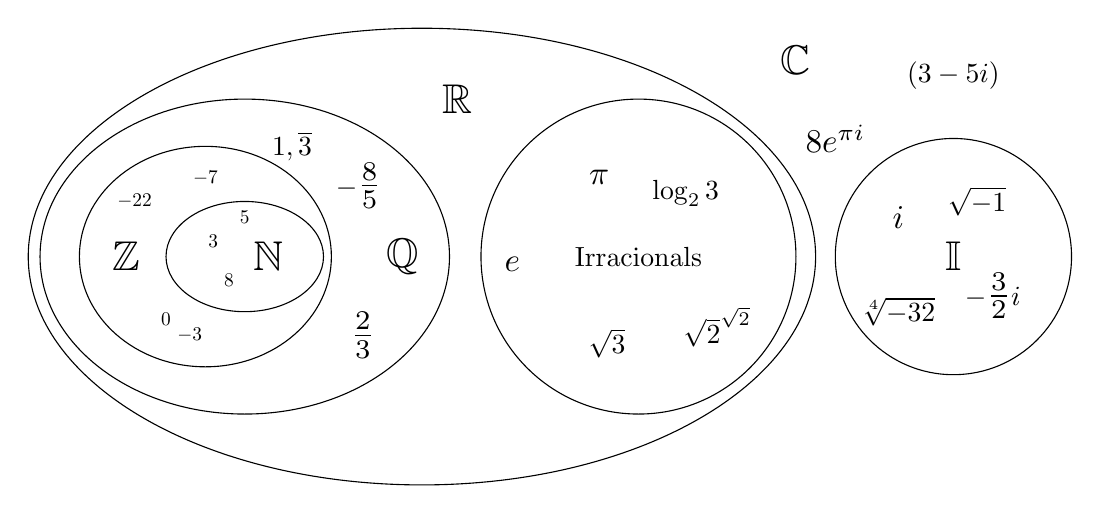
\begin{tikzpicture}
    %\draw[step=1cm,gray!15,very thin] (-5.9,-2.9) grid (8.9,2.9);

    % ELLIPSES:
    \draw (-1.5, 0) ellipse (1cm and 0.7cm);
    \draw (-2, 0) ellipse (1.6cm and 1.4cm);
    \draw (-1.5, 0) ellipse (2.6cm and 2cm);
    \draw (3.5, 0) ellipse (2cm and 2cm);
    \draw (.75, 0) ellipse (5cm and 2.9cm);
    \draw (7.5, 0) ellipse (1.5cm and 1.5cm);

    % LETERS:
    \draw (-1.2,0) node[anchor=center] {\scalebox{1.5}{$\mathbb{N}$}};
    \draw (-3,0) node[anchor=center] {\scalebox{1.5}{$\mathbb{Z}$}};
    \draw (0.5,0) node[anchor=center] {\scalebox{1.5}{$\mathbb{Q}$}};
    \draw (3.5,0) node[anchor=center] {Irracionals};
    \draw (1.2,2) node[anchor=center] {\scalebox{1.5}{$\mathbb{R}$}};
    \draw (7.5,0) node[anchor=center] {\scalebox{1.5}{$\mathbb{I}$}};
    \draw (5.5, 2.5) node[anchor=center] {\scalebox{1.5}{$\mathbb{C}$}};

    % NUMBERS:
    \draw (-1.9,0.2) node[anchor=center] {\scalebox{.7}{$3$}};
    \draw (-1.7,-0.3) node[anchor=center] {\scalebox{.7}{$8$}};
    \draw (-1.5,0.5) node[anchor=center] {\scalebox{.7}{$5$}};

    \draw (-2,1) node[anchor=center] {\scalebox{.7}{$-7$}};
    \draw (-2.5,-0.8) node[anchor=center] {\scalebox{.7}{$0$}};
    \draw (-2.9,.7) node[anchor=center] {\scalebox{.7}{$-22$}};
    \draw (-2.2,-1) node[anchor=center] {\scalebox{.7}{$-3$}};

    \draw (0,-1) node[anchor=center] {\scalebox{1.4}{$\frac{2}{3}$}};
    \draw (-.05,.9) node[anchor=center] {$-$\scalebox{1.4}{$\frac{8}{5}$}};
    \draw (-.9,1.4) node[anchor=center] {$1,\overline{3}$};

    \draw (3, 1) node[anchor=center] {\scalebox{1.2}{$\pi$}};
    \draw (3.1, -1.1) node[anchor=center] {$\sqrt{3}$};
    \draw (4.5, -.9) node[anchor=center] {\(\sqrt{2}^{\sqrt{2}}\)};
    \draw (1.9, -0.1) node[anchor=center] {\scalebox{1.2}{$e$}};
    \draw (4.1, 0.8) node[anchor=center] {$\log_2 3$};

    \draw (6.8, .5) node[anchor=center] {\scalebox{1.2}{$i$}};
    \draw (7.8, .7) node[anchor=center] {$\sqrt{-1}$};
    \draw (6.8, -.7) node[anchor=center] {$\sqrt[4]{-32}$};
    \draw (8, -.5) node[anchor=center] {$-$\scalebox{1.4}{$\frac{3}{2}$}$i$};

    \draw (6,1.5) node[anchor=center] {\scalebox{1.2}{\(8e^{\pi i}\)}};
    \draw (7.5,2.3) node[anchor=center] {$(3 - 5i)$};


    %\foreach \x in {-6,-5,-4,-3,-2,-1,0,1,2,3,4,5,6,7,8,9}
    %    \draw (\x cm,1pt) -- (\x cm,-1pt) node[anchor=north] {$\x$};
    %\foreach \y in {-3,-2,-1,1,2,3}
    %    \draw (1pt,\y cm) -- (-1pt,\y cm) node[anchor=east] {$\y$};

\end{tikzpicture}
}
Els nombres reals s'usen per mesurar quantitats reals, com ara longituds, velocitats, arees. I aquests nombres son suficients per a resoldre moltes equacions. Però existeixen algunes que simplement no es poden resoldre amb aquests numeros, com per exemple:
\[x^2 + 1 = 0 \; ; \; x = \pm\sqrt{-1}\]
No hi ha cap nombre que ens doni un resultat real per a \(\sqrt{-1}\). Sent aquest irreductible, li direm $i$, d'\textit{imaginary}.
\[\sqrt{-1} = i\]
Tenim, doncs, dues formes de representar els nombres complexos. La forma polar i la cartesiana, respectivament son: \newline \newline
\centerline{
\(
z = Me^{i\theta}
\left\{ \begin{array}{lcc}
        M \in \mathbb{R} \\
        \\ \theta \: en \: rad
         \end{array}
\right.\)
\(
\hspace*{6mm} ; \hspace*{6mm}
    z = a + bi
    \left\{ \begin{array}{lcc}
            a, b \in \mathbb{R}\\
            \\ bi \in \mathbb{I}
             \end{array}
   \right.
\)
}
%Aquesta forma ens indica l'angle directament en l'expressió i el seu módul. L'altra, en canvi, ens permet saver les seves "coordenades".
\subsubsection{El pla complex}
Si agafem la definició del nombre complex cartesià, tenim dues parts. La part real, $a$, i la part imaginaria, $bi$. D'aquesta manera podem mirar els nombres complexos com a punts o vectors, posant la part real en l'eix $x$ i en l'eix $y$ la part imaginaria. Per exemple:
\[z = 3 - 2i \; \rightarrow \; (3, -2)
\]
Així podem veure doncs que per a representar tots els nombres complexos podem utilitzar un pla. Si en aquest pla fem el que s'ha dit abans, l'$a$ en les $x$ i la $b$ en les $y$, hem creat el pla complex. \n
Representem uns quants nombres:
\[z_1 = 3 - 2i \; ; \; z_2 = 1 + 3i \; ; \; z_3 = -3 + 1i \; ; \; z_4 = 5e^{0,644i}\]
\newline
\centerline{
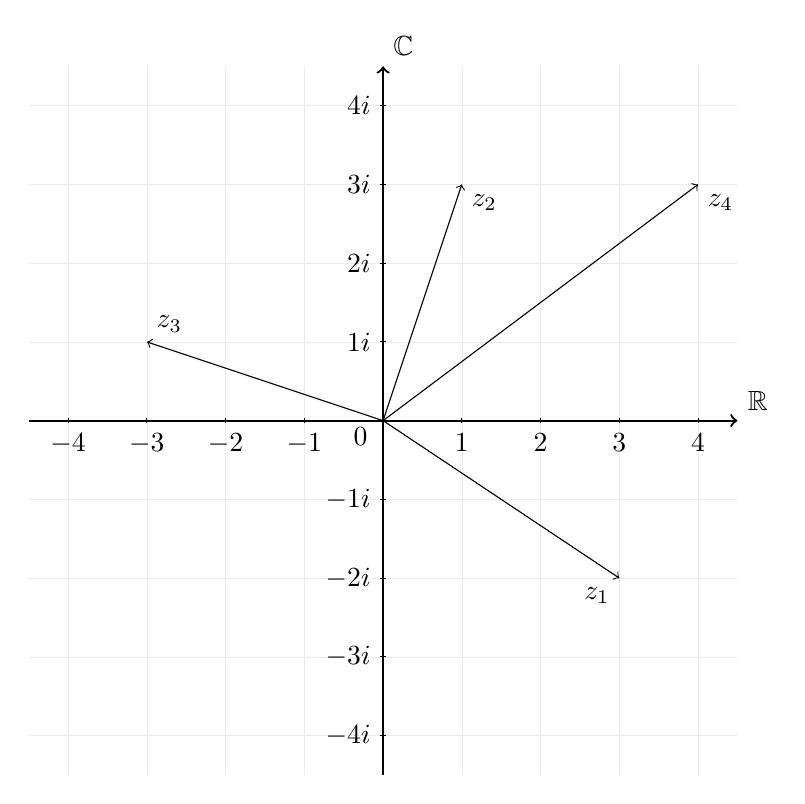
\begin{tikzpicture}
    \draw[step=1cm,gray!15,very thin] (-4.5,-4.5) grid (4.5,4.5);

    \draw[thick,->] (-4.5,0) -- (4.5,0) node[anchor=south west] {$\mathbb{R}$};
    \draw[thick,->] (0,-4.5) -- (0,4.5) node[anchor=south west] {$\mathbb{C}$};

    \draw (-0.5cm,1pt) node[anchor=north west] {$0$};

\foreach \x in {-4,-3,-2,-1,1,2,3,4}
    \draw (\x cm,1pt) -- (\x cm,-1pt) node[anchor=north] {$\x$};
\foreach \y in {-4,-3,-2,-1,1,2,3,4}
    \draw (1pt,\y cm) -- (-1pt,\y cm) node[anchor=east] {$\y i$};

    \draw[thin,->] (0,0) -- (3,-2) node[anchor=north east] {$z_1$};
    \draw[thin,->] (0,0) -- (1,3) node[anchor=north west] {$z_2$};
    \draw[thin,->] (0,0) -- (-3,1) node[anchor=south west] {$z_3$};
    \draw[thin,->] (0,0) -- (4,3) node[anchor=north west] {$z_4$};

\end{tikzpicture}
}

\subsection{Paral·lelització}
Quan programem, normalment el codi no és paral·lelitzat, doncs simplement li diem al processador que vagi fent línia a línia. Aquest mètode, quan tenim codi repetitiu, no és efficient. Seria millor si aquest codi repetitiu el poguessim executar multiples vegades a l'hora. Aquí és on entra la paral·lelització. \n
Aquesta la podem implementar de dues formes, per CPU o per GPU.
\subsubsection{CPU}
La CPU, \emph{Central Processing Unit}, és el component més important d'un ordinador. Seria com el cervell d'un animal. És que dona ordres a tothom. Aquesta compte amb diferents subprecessadors capaços de funcionar a l'hora i molt sovint es desaprofiten. \n
Estariem parlant d'uns pocs subporcessadors, en el meu cas en té 6. Però depen del processador, no hi ha un estàndar. \n
Per tant, seguint posant d'exemple el meu processador, podriem repetir la mateixa tasca 6 vegades a l'hora. Això ja ens dona molta aventatge. \n
Podriem estar temptants de dir que anirem 6 vegades més ràpid, però això no és així. L'acció d'enviar les dades per a realitzar el treball desitjat a un subprocessador consumeix temps, quan el subprocessador ha acabat ha de tornar les dades i s'han de sincronitzar tots els subprecessadors. Per tant, per a la realització de tasques petites no ens és eficient. \n
És útil quan volem realitzar tasques que consumeixin un temps gran.

\subsubsection{GPU}
La GPU, \emph{Graphics Processing Unit}, està enfocada en la idea de la paral·lelització. Aquesta unitat no es troba en tots els dispositius, ja que és prescindible, però molt útil. Originalment aquesta unitat va ser creada en la búsqueda de la rapidesa pel processament de cada píxel. Doncs és molt útil en videojocs i la generació de gràfics. \n
Últimament s'han trobat molt més usos d'aquesta unitat, com ara l'entrenament de \emph{Machine Learning} o la mineria de \emph{cryptomonedes} per exemple. \n
Al estar enfocada en aquesta idea de processar cada píxel, en el meu cas, té 1024 subprocessadors. Aquests son més petits que els de la CPU, per això hi han tants, però més eficients. \n
Aquest útlim ens serà útil en el càl·lcul de fractals.


\section{Historia}
Text històric.


\section{Tipus de fractals}
Dins de les fractals tenim diferents tipus, en podem destacar tres: les fractals naturals, les geomètriques i les algebraiques.

\subsection{Les fractals naturals}
Aquestes fractals es caracteritzen pel fet que apareixen a la natura. No segueixen cap forma geomètrica ni cap norma, simplement cada cop que ens apropem podem veure com es va repetint.
\newline

\begin{figure}[h]
    \centering
    \begin{minipage}{.5\textwidth}
      \centering
      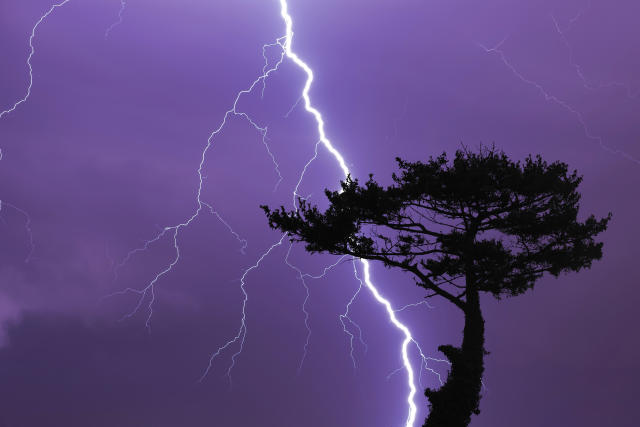
\includegraphics[width=.8\linewidth]{imatges/dos-fractals-naturals.jpg}
      \captionof{figure}{Un arbre i un llampec.}
      \label{fig:arbre_i_llampec}
    \end{minipage}%
    \begin{minipage}{.5\textwidth}
      \centering
      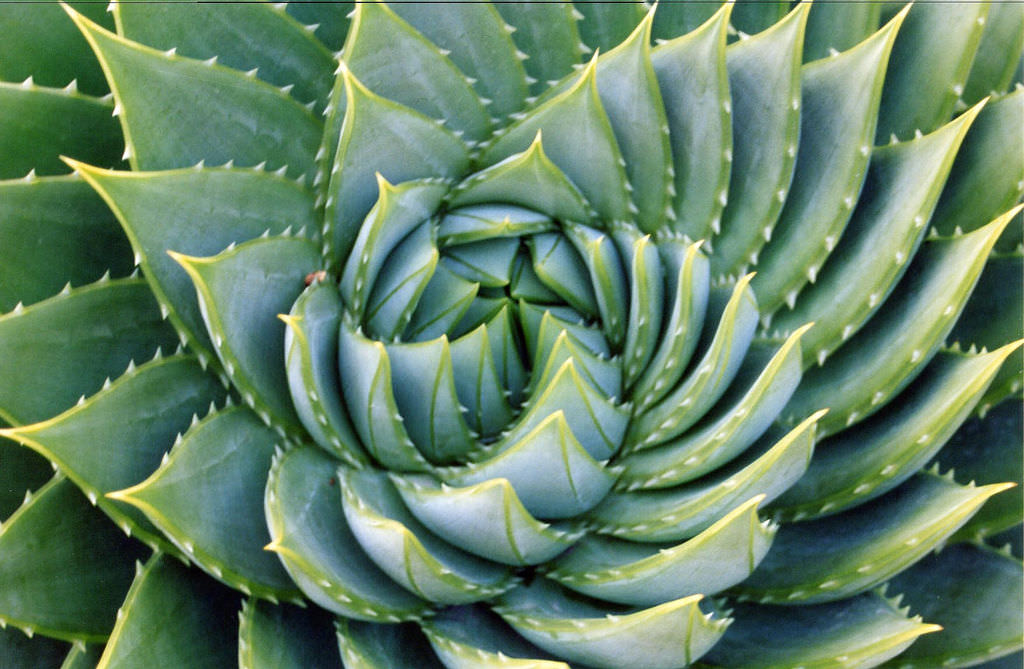
\includegraphics[width=.8\linewidth]{imatges/planta-espiral.jpg}
      \captionof{figure}{Planta creixent en espiral.}
      \label{fig:espiral}
    \end{minipage}
\end{figure}
\noindent
Com a exemples tenim l'arbre i el llampec en la figura \ref{fig:arbre_i_llampec}. Però a més a més, en la figura \ref{fig:espiral} podem veure una planta que creix en espiral. Aquesta segueix la Seqüència de Fibonacci i es pot veure com un cas especial de similitud amb ella mateixa.

\subsection{Les fractals geomètriques}
Aquestes fractals són els més senzills d'entendre, ja que simplement són ells mateixos repetits. Segueixen unes normes molt bàsiques, que canvien en cada fractal, i podem dir amb seguretat que no han estat generats arbitràriament, cosa que no podem estar tan segurs de pensar en les fractals algebraiques. \n
L'única diferència que hi ha entre una fractal geomètrica i una d'algebraica és el seu punt de partida. Doncs aquests s'inicien amb una forma geomètrica. \n
En la figura \ref{fig:sierpinski} podem veure el triangle de Sierpinski. El seu punt inicial és un triangle equilàter. Aquest triangle està ple i és emplenat amb un altre triangle equilàter buit al centre de la manera que aquest triangle sigui igual de gran que els tres triangles que es formen al seu costat. \n
En canvi, en la figura \ref{fig:arbre_fractal} podem veure una fractal en forma d'arbre. Aquest ha estat generat agafant una figura inicial en forma de Y i posant-hi, en la bifurcació d'aquesta figura, la mateixa, de mode que el tronc del model agregat és també la bifurcació de la figura inicial. Si aquesta acció és repetida suficients vegades per a no notar ja un canvi, tindrem la figura \ref{fig:arbre_fractal}.

\begin{figure}[h]
    \centering
    \begin{minipage}{.5\textwidth}
      \centering
      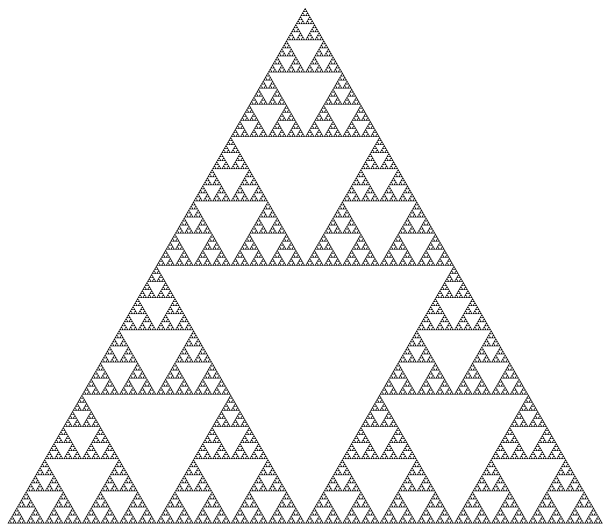
\includegraphics[width=.8\linewidth]{imatges/sierpinski.jpg}
      \captionof{figure}{Triangle de Sierpinski.}
      \label{fig:sierpinski}
    \end{minipage}%
    \begin{minipage}{.5\textwidth}
      \centering
      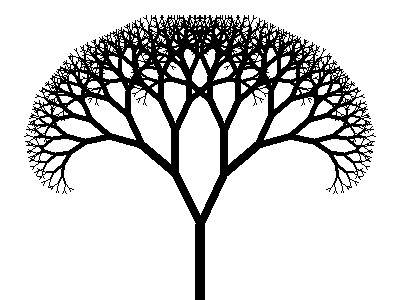
\includegraphics[width=.8\linewidth]{imatges/fractal-tree.jpg}
      \captionof{figure}{Fractal en forma d'arbre.}
      \label{fig:arbre_fractal}
    \end{minipage}
\end{figure}
\noindent

\subsection{Les fractals algebraiques}
Aquestes fractals, tal i com he anomenat abans, podriem pensar que han estat generades arbritàriament si ens limitem a veure una imatge. Aquestes fractals no son més que una equació de nombres complexos iterada infinitament. Si al posar un número del pla complex aquest no tendeix a infinit, aquest nombre forma part de la fractal. \n
Les fractals algebraiques no es limiten a una simple equació. També tenen les seves normes. Com ara començar a iterar el nombre igualant $z_0 = 0$ i fent que $c = v_{punt}$. Si l'equació d'aquesta fractal és $f(z) = z^2 + c$, s'anomena Conjunt de Mandelbrot.

\subsubsection{Conjunt de Mandelbrot}
Seguint amb l'exemple anterior, diguem que volem calular el nombre $z = -1 + 0i$ (si els nombres complexos no tenen part imaginaria, com aquest cas, els podem tractar com a nombres reals):
\[f(0) = 0^2 + c \; c = (-1, 0)\]
\[f_0(0) = 0^2 - 1 = -1\]
\[f_1(-1) = (-1)^2 -1 = 0\]
\[f_2(0) = 0^2 - 1 = -1\]
Com es pot veure, ja que el nombre no tendeix a infinit, doncs va saltant de 0 a -1, el nombre complex $z = -1 + 0i$, forma part del conjunt de Mandelbrot. Donant el nombre $z = 1 + 0i$:
\[f_0(0) = 0^2 + 1 = 1\]
\[f_1(1) = 1^2 + 1 = 2\]
\[f_2(2) = 2^2 + 1 = 5\]
\[f_3(5) = 5^2 + 1 = 26\]
Amb aquest nombre no hem tingut tanta sort! Cada com que iterem aquest nombre es fa cada cop més i més gran. Això ens indica que aquest nombre tendeix a infinit. Per tant, no forma part del confunt de Mandelbrot. Si fem això per cada punt, obtenim aquesta imatge:

\begin{figure}[h!]
    \centering
    
\includegraphics[width=.65\linewidth]{imatges/Captured_On_Sat_Aug__7_16-04-10_2021-.jpg}
    \captionof{figure}{Representació del conjunt de Mandelbrot.}
    \label{fig:mandelbrot_example}
\end{figure}

\subsubsection{Conjunt de Julia}
El conjunt de Julia segueix la mateixa funció que el de Mandelbrot. Però en aquest cas canviem la norma. Fixem $c$ a un nombre arbritari que nosaltres escollim i canviem $z_0$ pel punt on s'està iterant. Donem un exemple, tractarem amb nombres reals, doncs és més senzill:
\[c = 1 + 0i\]
Donem els punts $z_{0_1} = 1 + 0i$ i $z_{0_2} = -1 + 0i$: \newline
\begin{center}
\begin{tabularx}{0.8\textwidth} {
  >{\centering\arraybackslash}X |
  >{\centering\arraybackslash}X}
  \(f_{1_1}(z_{0_1}) = 1^2 + 1 = 2\) \vspace*{3mm} & \(f_{2_1}(z_{0_2}) = (-1)^2 + 1 = 2\) \\
  \(f_{1_2}(2) = 2^2 + 1 = 5\) \vspace*{3mm} & \(f_{2_2}(2) = 2^2 + 1 = 5\) \\
  \(f_{1_3}(5) = 5^2 + 1 = 26\) & \(f_{2_3}(5) = 5^2 + 1 = 26\)
\end{tabularx}
\end{center}
\noindent \newline
En aquest cas podem veure com els dos nombres no formen part del conjunt de Julia per $c = 1 + 0i$. \n
Fixem $c$ a un altre nombre:
\[c = -1 + 0i\]
Donem els mateixos punts $z_{0_1} = 1 + 0i$ i $z_{0_2} = -1 + 0i$: \newline
\begin{center}
\begin{tabularx}{0.8\textwidth} {
  >{\centering\arraybackslash}X |
  >{\centering\arraybackslash}X}
  \(f_{1_1}(z_{0_1}) = 1^2 - 1 = 0\) \vspace*{3mm} & \(f_{2_1}(z_{0_2}) = (-1)^2 + 1 = 0\) \\
  \(f_{1_2}(0) = 0^2 - 1 = -1\) \vspace*{3mm} & \(f_{2_2}(0) = 0^2 - 1 = -1\) \\
  \(f_{1_3}(-1) = (-1)^2 - 1 = 0\) & \(f_{2_3}(-1) = (-1)^2 - 1 = 0\)
\end{tabularx}
\end{center}
\noindent \newline
Ara podem veure que els dos nombres formen part del conjunt de Julia per $c = -1 + 0i$. \n
Si ho fesim per cada punt del pla obtindriem aquestes imatges:
\begin{figure}[h]
    \centering
    \begin{minipage}{.5\textwidth}
      \centering
      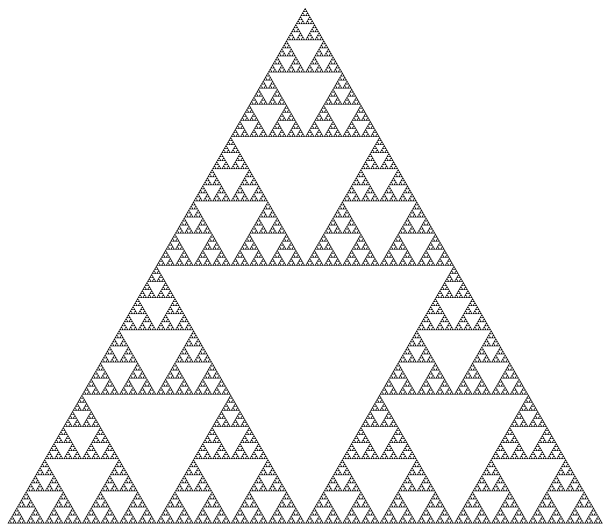
\includegraphics[width=.8\linewidth]{imatges/sierpinski.jpg}
      \captionof{figure}{Per $c = $.}
      \label{fig:Julia_example_}
    \end{minipage}%
    \begin{minipage}{.5\textwidth}
      \centering
      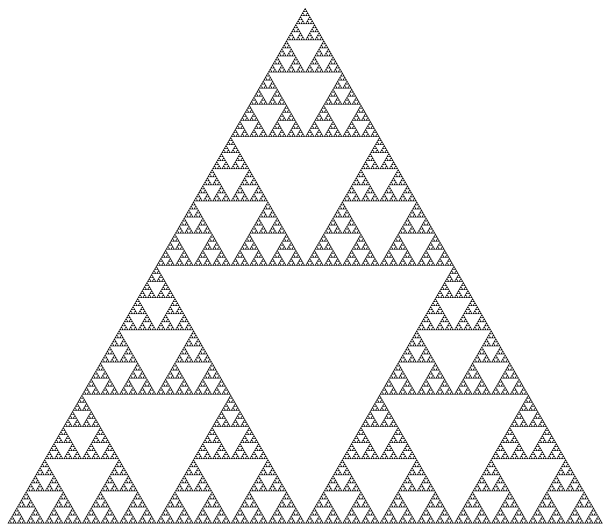
\includegraphics[width=.8\linewidth]{imatges/sierpinski.jpg}
      \captionof{figure}{Per $c = $.}
      \label{fig:Julia_example_}
    \end{minipage}
\end{figure}
\noindent


\section{Programari}
El programari creat en aquest projecte té la finalitat de representar el fractal $f(z) = z^2 + c$, llavors, sabent que necessitarem rapidesa de computació, ja que volem que no vagi massa lent, he utilitzat C++. Aquest llenguatge de programació és un dels més ràpids que existeix actualment. Aquest llenguatge és una ampliació de C derivat a objectes, per tant, la programació és més intuïtiva.

\subsection{Representació de la fractal}
Per a la representació del fractal, utilitzarem una llibreria per a poder mostrar el que estem calculant. Aquesta llibreria es diu olcPixelGameEngine. He escollit aquesta llibreria perquè s'encarregui de la visualització per un simple motiu, que es pot tractar cada píxel per individual. \n
En poder tractar cada píxel com un sol, podem tractar-ho com punts d'un mapa bidimensional. És a dir, cada píxel representa un punt en el pla dels complexos.
\subsubsection{Tractament dels píxels}
Per accedir a cada píxel hem d'anar del 0 al 1920 per als punts d'esquerra a dreta i de 0 al 1080 per als punts de dalt a baix. Això és un problema tenint en compte que la fractal va del $-2$ a l'$1$ i del $-1$ a l'$1$ respectivament. Però aquests números han de ser arbitraris, ja que si volem apropar-nos, aquests canviaran. Per tant, hem d'idear una solució que ho tingui en compte.\n
Bé, per passar de les coordenades de l'ordinador a les de la fractal o a les coordenades que nosaltres volem, hem de normalitzar les coordenades de l'ordinador, perquè vagin de $0$ a $1$ en comptes de $0$ a $1920$ o $0$ a $1080$. Per fer-ho simplement dividirem la coordenada que ens arriba pel nombre total de punts que hi ha. \n
Segon, haurem de saber l'espai que hi ha d'extrem a extrem dins de la fractal. Per saber-ho simplement restarem els extrems per saber la distància i com que ens és igual l'ordre, ho passarem per un absolut perquè ens doni una solució positiva sempre. \n
Finalment, per l'eix de les $x$, agafarem l'extrem de l'esquerra (el més petit) i li sumarem el valor normalitzat multiplicat per l'espai total de les $x$. En el cas de l'eix de les $y$, farem el mateix, però agafarem el valor de dalt i li restarem el valor normalitzat per les $y$ multiplicat per l'espai. \n
Aquesta suma i resta no són arbitràries, la suma la fem perquè els nombres que rebem van d'esquerra a dreta augmentant amb l'eix d'abscisses i volem que vagi igual en la fractal, però van d'amunt en avall en l'eix d'ordenades i en la fractal van a l'inrevés, per això es resta. \n
Haig d'aclarir que aquest tractament només es fa servir en canviar de posició, per al càlcul de la fractal s'utilitza una altra manera igual de vàlida, però canvia una cosa, en l'altre l'hi hem de dir en cada punt on es troba de les coordenades de l'ordinador, en aquesta no. Ja que al principi calcula, restant i fent l'absolut dels extrems i llavors dividint per l'altura o l'allargada de l'ordinador i llavors quan acaba d'una posició suma o resta aquest valor a una variable que ens indica la posició en la qual es troba. Aquesta manera és més directe i computacionalment és una simple suma. \n
Es fan servir les dues, ja que a l'hora de fer el càlcul es necessita rapidesa i a l'hora d'apropar-nos necessitem un punt només.

\subsubsection{Càlcul de la fractal en sí}
Com ja sabem cada punt de la fractal, perquè l'hem calculat en el problema anterior, i també sabem que podem tractar els nombres complexos com a dos nombres, així:
\[z = a + bi\]
\[z = x + yi\]
\centerline{(Sent x, y els valors en cada punt)}
\[z^2 = (x + yi)^2\]
Si ho desenvolupem tenim:
\[z^2 = x^2 + 2xyi + (yi)^2\]
\[z^2 = (x^2 - y^2) + (2xy)i\]
Per tant, sabem quina part del nombre complex serà la real i quina la imaginaria, per tant ho podem desarrollar dient que:
\[z_\mathbb{R} = x^2 - y^2\]
\[z_\mathbb{C} = 2xy\]
Podem fer el mateix per $c$. \n
Així doncs és molt més fàcil de programar, simplement hem de fer unes multiplicacions, sumes i restes. \n
Un cop sabem com determinar cada part, la real i la imaginaria, és hora de calcular-ho. Aquest conjunt, el de Mandelbrot, es calcula posant $z_0 = 0$ i $c$ igual al punt, llavors s'itera un nombre infinit de vegades $z$ en la funció $f(z) = z^2 + c$. Com que no tenim infinit temps, iterarem un nombre finit de vegades i anirem augmentant aquestes iteracions perquè sigui més precís.
\subsubsection*{Determinar quan un punt senvà al infinit}
Per determinar-ho, hem de saber si $|z| > 2$. Aquesta comprovació podem fer-la amb el teorema de Pitàgores:
\[|z| = \sqrt{x^2 + y^2}\]
Per estalviar recursos i no haver de fer l'arrel quadrada cada cop que calculem una iteració d'un punt del pla, farem:
\[|z|^2 = x^2 + y^2 > 2^2\]
Per tant:
\[|z|^2 > 4\]
Quan aquesta inequació es compleixi, deixarem d'iterar el punt i retornarem un valor del 0 al 1, determinat per aquesta operació: $v = k / n$, sent $v$ el valor tornat, $k$ la iteració on ha parat i $n$ el nombre total d'iteracions.\n
En el cas que la inequació no es compleixi i $k = n$ retornarem 0. \n
D'aquesta manera, veurem representat les voreres de la fractal, simplement una decisió artística.
\subsubsection{Dibuix de la fractal}
Per a pinar el fractal simplement accedirem a la matriu on està cada valor $v$ de cada punt i el pintarem. He escollit el color(r, g, b): (255, 163, 119) o \#FFA377, per tant direm que:
\[color_{punt} = (255 - (255 - 255) \cdot v, 255 - (255 - 163) \cdot v, 255 - (255 - 119) \cdot v)\]
\subsubsection*{Resultat inicial}
Si apliquem tot el que hem dit en aquesta part, tindrem el següent resultat:
%Captured_On_Sat_Aug__7_16-05-37_2021-.jpg
\begin{figure}[h!]
    \centering
    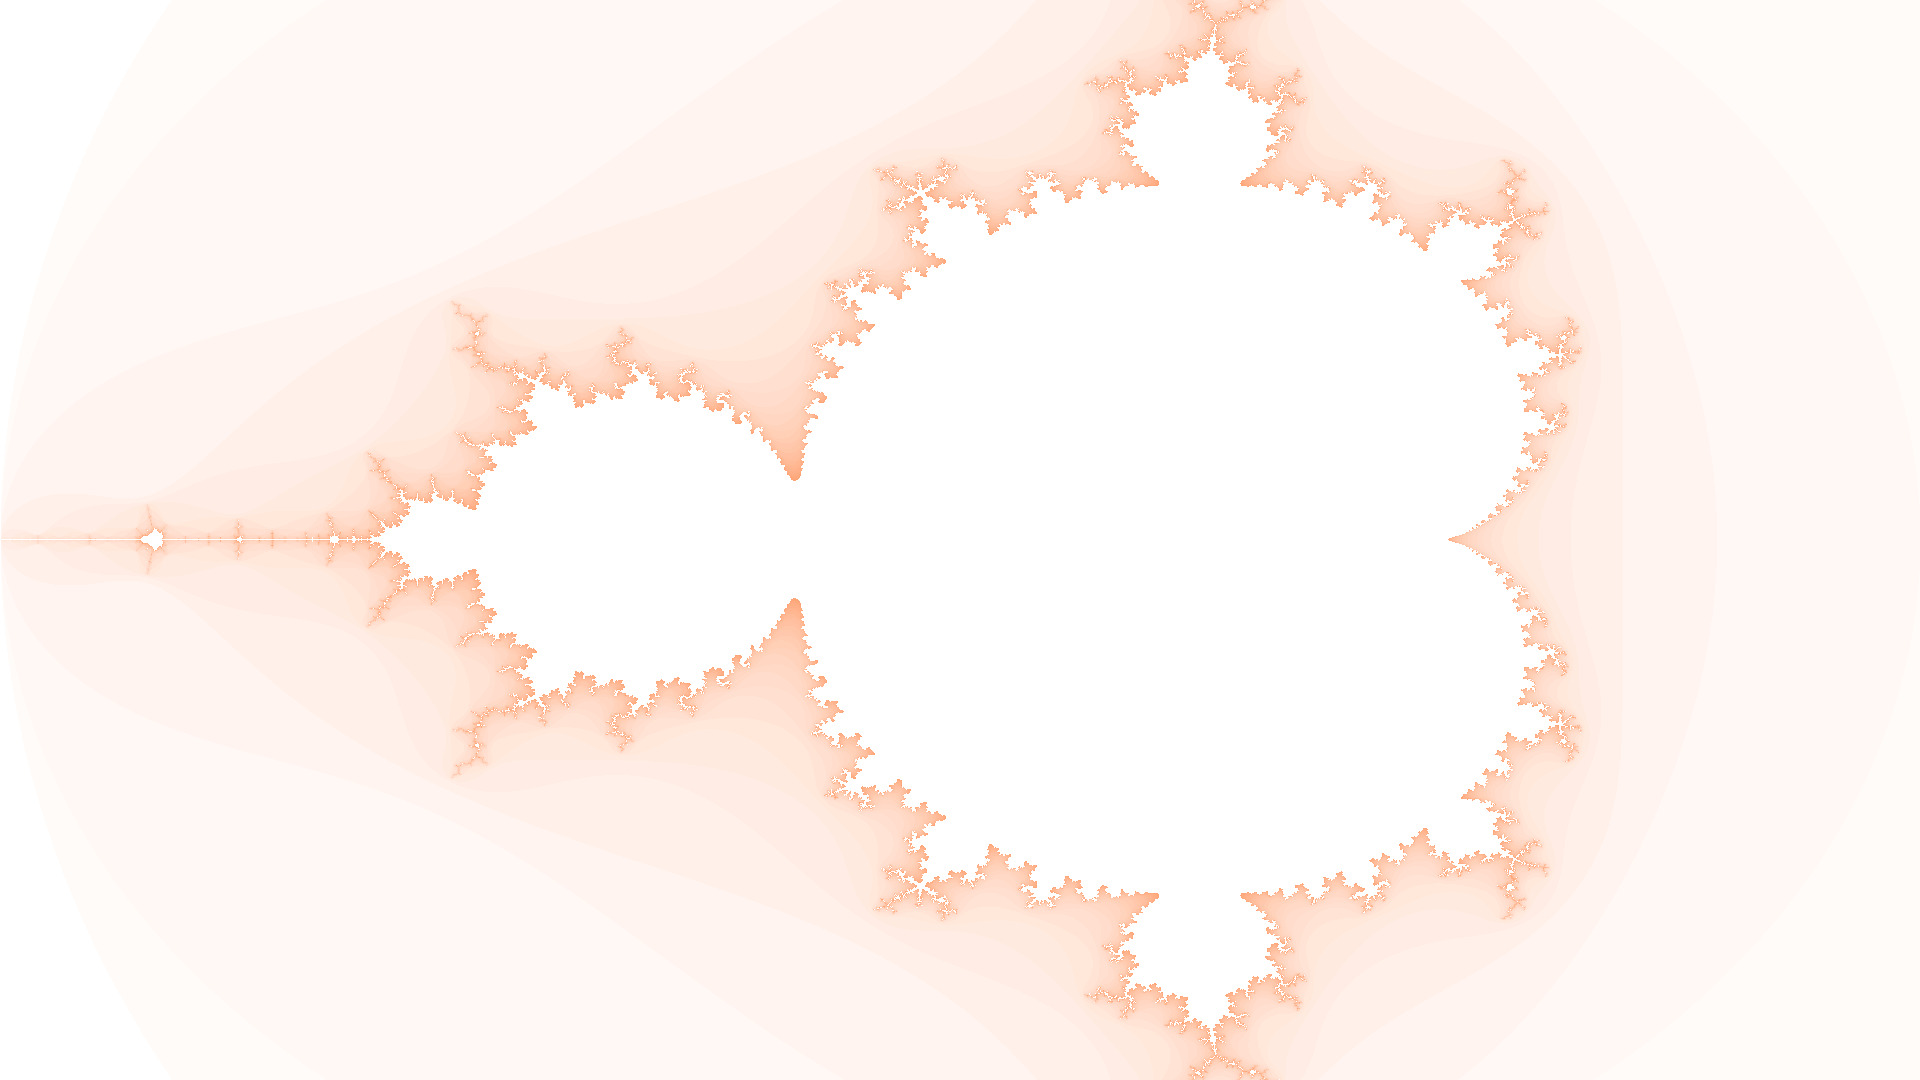
\includegraphics[width=.65\linewidth]{imatges/Captured_On_Mon_Dec__6_18-48-29_2021-.jpg}
    \captionof{figure}{Imatge capturada el 7 d'Agost de 2021 sense ampliacions.}
    \label{fig:resultat_inicial}
\end{figure}
\n \noindent
Jugant amb els colors podem generar imatges com aquesta:
%Captured_On_Sat_Aug__7_16-04-10_2021-.jpg
\begin{figure}[h!]
    \centering
    
\includegraphics[width=.65\linewidth]{imatges/Captured_On_Sat_Aug__7_16-04-10_2021-.jpg}
    \captionof{figure}{}
    \label{fig:jugant_amb_colors}
\end{figure}
\n \noindent
En la figura \ref{fig:jugant_amb_colors}, en comptes de retornar un número del 0 a l'1, es retorna un número del 0 al 255 i se segueix aplicant els colors com hem vist abans, d'aquesta manera, en arribar al número més gran, diguem que multipliquem que ens retorna un dos, en aquest cas es faria (pel blau) $color_{blau} = 163 \cdot 2 = 326$. Aquest és un valor massa gran per aplicar-ho als colors, que van fins al 255. Per tant, es resta 255 al color, és a dir, 71. Llavors, el valor del color blau seria 71.

\subsection{Ampliació}
Per que sigui més interesant el fet de crear aquest programa, farem que pugui ampliar cap a la part que nosaltres volguem. \n
L'ampliació es farà quan l'usuari premi qualsevol punt de la pantalla i arrossegui el cursor fins on vulgui. \n Per a que la tria del lloc sigui més visual, dibuixarem un rectangle al lloc on s'ampliarà. \n
Bàsicament direm, quan el botó esquerra del cursor hagi estat pres, guardarem aquestes coordenades, que aniran de 0 a 1920 i de 0 a 1080, i quan es deixi de premer i estigui a un altre lloc suficientment lluny, a uns 30 píxels, llavors "guardarem" les coordenades finals del cursor.
\subsubsection{Tractament de les coordenades finals del cursor}
"Guardarem" ja que no volem que ens quedi la pantalla estirada: \n
Posar imatge. \n
Perque la pantalla no quedi estirada simplement hem de mantenir l'\emph{Aspect Ratio}. I que és això? Doncs es básicament els píxels d'amplada dividits pels d'altura. L'estandar ara mateix és 16:9, és a dir, per cada 16 píxels que hi ha d'amplada hi ha 9 d'altura. Sabent aquesta definició és senzill doncs saber a quin lloc correspondria l'altura final en relaició a la amplada que estem recorrent amb el cursor. \n
Sabent que la nostra pantalla és de 16:9:
\[\frac{16}{9} = \frac{amplada}{altura}\]
Sabem l'amplada (posició del cursor en X), ens interesa l'altura:
\[altura = \frac{9 \cdot amplada}{16}\]
Doncs ja la tenim. Es senzill.
\subsubsection{Ampliació en sí}
Fent us de la funció que hem creat abans, per saber quina coordenada li correspon al fractal donant-li una coordenada del cursor, li donem els punts que ens han sortit, i, depenent de la posició final del cursor, si està més adalt, més a l'esquerra, més abaix, les igualem a les variables dels límits. \n
Llavors, si fem que just després s'actualitzi la fractal, aquesta s'ampliarà.


%\section{Per qué quan $|z_N| > 2$ ja diem que $z \rightarrow \infty$?}
...


\section{Reducció del temps}
Sí augmentem una barbaritat les iteracions, diguem 10000, el temps de càlcul augmenta, no linealment, sino exponencialment. \n
Això ho podem veure experimentalment:

\subsection{Per CPU}
Tractarem de paral·lelitzar amb la CPU. Tal i com he explicat abans, la CPU té diferents subprocessadors i els podem utilitzar tots a l'hora. \n
Utilitzarem la llibreria \emph{openmp}. És molt fàcil de fer servir, és una simple linea de codi i ajustar un parametre. \n
Aquí aniran algunes estimacions de quan de temps ens podem estalviar si utilitzaem la llibreria. \n
Amb aquesta llibreria no només paral·lelitzarem el càlcul de la fractal, també paral·lelitzarem el dibuix d'aquesta. Al fer-ho, tindrem una ventatge de - segons.

\subsection{Per GPU}
Aquesta paral·lelització disminuirà molt el temps de càlcul. Però no és tan senzill com la paral·lelització amb la CPU. \n
Utilitzarem CUDA, el qual ja no és una llibreria, si no és una extensió del lleguatge de programació C. Aquesta extensió ens permetrà accedir automàticament als subprocessadors. \n
Però no és tan senzill. Hi ha disponibles 1024 subprocessadors, els quals no és necessari utilitzar tots a l'hora però ho farem així perque volem la màxima eficiencia. \n
Tenim 1920x1080 punts. Hem d'accedir a cada un per saber la seva posició. Però no podem anar sumant 1 com feiem abans, perquè això només ho podem fer amb programació en serie. Per tant, el métode escollit serà aquest:
\begin{center}
    Si tenim 1024 subprocessadors i una graella d'\emph{AMPLADA}x\emph{ALTURA}, al total li direm $N$, per cada subprocessador agafarem un bucle que vagi fins a $N$ i començarem el bucle per l'identificador de cada subprocessador (ens donarà un nombre de l'1 al 1024), llavors, cada vegada que el bucle acabi, sumarem 1024. Així ens donarà un número únic en cada iteració del bucle i en cada subprocessador. Al fer aquest proscés, tindrem una graella semblant a aquesta (molt més gran, clar):
\end{center}

\centerline{
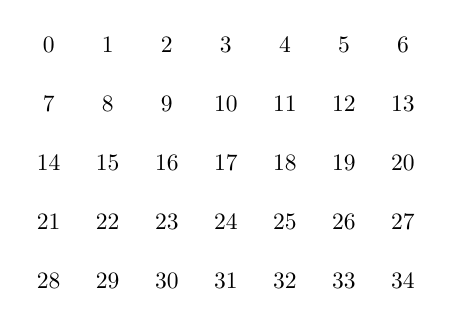
\begin{tikzpicture}
\foreach \x in {-2.25,-1.5,-0.75,0,0.75,1.5,2.25}
    \foreach \y in {-1.5,-0.75,0,0.75,1.5}
        \pgfmathtruncatemacro{\xy}{-(-\x*4/3+7*\y*4/3) + 17)}
        \draw (\x cm,\y cm) -- (\x cm,\y cm) node[anchor=center] {\scalebox{0.85}{\xy}};

\end{tikzpicture}
}

\begin{center}
    Agafarem el valor únic anterior i farem la divisió euclidiana, el divisor serà l'amplada, el quocient serà la posició $y$ i el residu la posició $x$. Això és més fàcil dir-ho que demostrar-ho. Per fer-ho, farem us de la graella anterior de 7x5.
\end{center}
\begin{center}
    Si ens hi fixem en un punt, diguem el 17, podem dir que el punt amb coordenades ($x$, $y$) és (2, 3), a ull, considerant el punt 0 com a (0, 0).
\end{center}
\centerline{
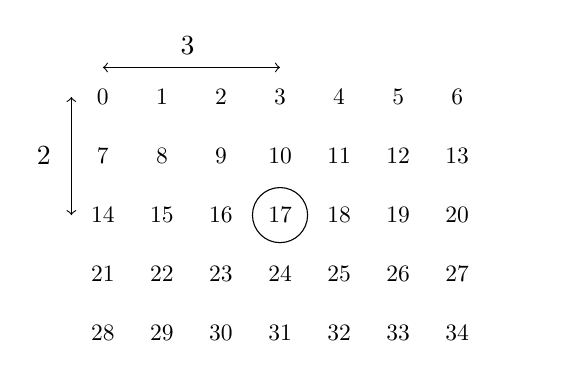
\begin{tikzpicture}
% El punt 17 té les coordenades:
% 0, 0

\draw [thin, to-to](-2.25,1.875) -- (0,1.875);
\draw [thin, to-to](-2.65,1.5) -- (-2.65,0);
\draw (0,0) circle (0.35);
\draw (-1.175, 2.15) node[anchor=center] {3};
\draw (-3, 0.75) node[anchor=center] {2};

\draw [thin, to-to, color=white](2.65,-1.5) -- (2.65,0);
\draw [color=white](3, -0.75) node[anchor=center] {2};


\foreach \x in {-2.25,-1.5,-0.75,0,0.75,1.5,2.25}
    \foreach \y in {-1.5,-0.75,0,0.75,1.5}
        \pgfmathtruncatemacro{\xy}{-(-\x*4/3+7*\y*4/3) + 17)}
        \draw (\x cm,\y cm) -- (\x cm,\y cm) node[anchor=center] {\scalebox{0.85}{\xy}};


\end{tikzpicture}
}

\begin{center}
    Podem veure que per passar una casella cap a baix, és a dir, augmentar la $y$ en 1, hem de sumar 7. Aquest 7 no és arbritari, és l'amplada. Si volem anar una casella amunt, disminuir la $y$ en 1, hem de restar 7, el que és el mateix l'amplada. En canvi, si volem moure'ns per les $x$\'s, llavors simplement hem d'augmentar o disminuir 1. Per tant, si dividim el nombre de la casella per l'amplada i obtenim el residu, obtenim el nombre en sí:
\end{center}

\centerline{\opidiv{17}{7}}

\begin{center}
    Com hem vist abans, el divisor és l'amplada, el quocient és l'ordenada $y$ i el residu l'ordenada $x$. S'ha de dir que aquest resultat no ens dona les coordenades en la fractal, si no ens dona en coordenades del cursor. Simplement ho passem per la funció creada anteriorment per passar-ho.
\end{center}

\noindent Les parts que es diferèncien del codi de CUDA i el codi amb C++ es troben a la pàgina \pageref{app:CUDA}, dins de l'Annex. \n
Amb CUDA no paral·lelitzarem el dibuix de la fractal, tal i com hem fet a l'anterior. Això és degut a que el temps de sincronització és més alt que el temps que el temps de càlcul en paral·lel amb la CPU. Així doncs, ho deixarem així. Per tant, mesclarem les dues i ens donarà el resultat més eficient. Sempre parlant de l'aplicació del conjunt de Mandelbrot. \n

\noindent En l'aplicació del conjunt de Julia, el càlcul en paral·lel, primerament no resulta beneficiòs. Ja que per comunicar amb la gràfica ja tarda més, en alguns casos, que el càlcul en serie.

\subsubsection{A vegades no és tan eficient, conjunt de Julia}
He recopilat algunes dades per veure aquesta pèrdua d'eficiéncia. Ja sabem què causa aquesta ineficiència però em resulta interessant comentar aquestes dades. \n
Les dades són el temps que tarda en fer el càlcul de la fractal i anem girant c. Tenim un total de 360 dades, una per cada grau que fem girar c. Aquesta comença amb una magnitud de ... i a 0 graus. Totes les dades es troben a l'Annex, pàgina \pageref{app:Julia_times}.


\section{Augmentant els límits}

\subsection{Presició de l'ordinador}
Si ens apropem molt a dins del fractal podem veure que tenim uns límits. Aquests límits estan deguts a que l'ordinador no té una presició infinita. Tampoc està inclosa en C++, en canvi si que està incorporada en Python.


\subsection{Presició arbitraria}
En un intent d'augmentar els límits, o simplement eliminar-los, he creat una llibreria de presició casibé infinita.

Maleuradament aquesta llibreria no està optimitzada.


\appendix
\section{Annex}

El codi del programari complert utilitzat està a GitHub. Des d'allà podreu accedir a les diferentes versions del programari: \n
   - El conjunt de Mandelbrot;\n
   - El conjunt de Julia;\n
   - El conjunt de Mandelbrot amb CUDA;\n
   - El conjunt de Julia amb CUDA.\n
Els executables també es troben a GitHub (veure arxius amb la terminació .exe). \n


\noindent Aquestes son les parts més interessants del codi utilitzat:
\label{app:CUDA}
\lstset{belowcaptionskip=1\baselineskip,
    breaklines=true,
    language=C++,
    showstringspaces=false,
    basicstyle=\footnotesize\ttfamily,
    keywordstyle=\bfseries\color{green!40!black},
    commentstyle=\itshape\color{purple!40!black},
    stringstyle=\color{orange},
    numberstyle=\color{codegray},
    tabsize=2,
    numbers=left,
    numbersep=5pt,
}
% Que loco. Posar el codi de CUDA que interesi.
\lstinputlisting[language=C++, firstline=62, lastline=91, firstnumber=62]{main.cpp}
\noindent Codi de CUDA: \n

\subsection*{El temps de càlcul del conjunt de Julia}
\label{app:Julia_times}
La magnitud de c és de ... . \n \newline
\twocolumn
\begin{supertabular}{|c|c|c|}
  \hline
  \scalebox{0.8}{angle (rad)} & \scalebox{0.8}{serie (s)} & \scalebox{0.8}{paral·lel (s)} \\ \hline

  0 & 0.0106577	& 0.0113933 \\ \hline
0.0174533 & 0.0114426	& 0.0133066 \\ \hline
0.0349066 & 0.0098439	& 0.0132896 \\ \hline
0.0523599 & 0.0098563	& 0.0268698 \\ \hline
0.0698132 & 0.0099874	& 0.013067 \\ \hline
0.0872665 & 0.0097958	& 0.0136759 \\ \hline
0.10472 & 0.0098975	& 0.0129127 \\ \hline
0.122173 & 0.0099488	& 0.0132821 \\ \hline
0.139626 & 0.009987	& 0.0129455 \\ \hline
0.15708 & 0.0105209	& 0.0132805 \\ \hline
0.174533 & 0.0098963	& 0.0133045 \\ \hline
0.191986 & 0.0099542	& 0.0132887 \\ \hline
0.20944 & 0.0102923	& 0.01328 \\ \hline
0.226893 & 0.0103477	& 0.0128789 \\ \hline
0.244346 & 0.0099877	& 0.0132876 \\ \hline
0.261799 & 0.0100088	& 0.0132195 \\ \hline
0.279253 & 0.0100336	& 0.0133624 \\ \hline
0.296706 & 0.0101255	& 0.0133695 \\ \hline
0.314159 & 0.010392	& 0.012938 \\ \hline
0.331613 & 0.0100522	& 0.0133455 \\ \hline
0.349066 & 0.0100205	& 0.0133377 \\ \hline
0.366519 & 0.0107418	& 0.0138779 \\ \hline
0.383972 & 0.010152	& 0.0133971 \\ \hline
0.401426 & 0.0104101	& 0.0131703 \\ \hline
0.418879 & 0.0101925	& 0.0134293 \\ \hline
0.436332 & 0.0102656	& 0.0130404 \\ \hline
0.453786 & 0.0102312	& 0.0133713 \\ \hline
0.471239 & 0.0103227	& 0.0131125 \\ \hline
0.488692 & 0.0103432	& 0.0134278 \\ \hline
0.506146 & 0.0105893	& 0.0134783 \\ \hline
0.523599 & 0.0112319	& 0.0135018 \\ \hline
0.541052 & 0.0105767	& 0.013527 \\ \hline
0.558505 & 0.0105779	& 0.0131717 \\ \hline
0.575959 & 0.0109517	& 0.0136023 \\ \hline
0.593412 & 0.0106392	& 0.0135628 \\ \hline
0.610865 & 0.010704	& 0.0135926 \\ \hline
0.628319 & 0.0110706	& 0.0132919 \\ \hline
0.645772 & 0.0108559	& 0.0138484 \\ \hline
0.663225 & 0.0109403	& 0.0135152 \\ \hline
0.680679 & 0.0110029	& 0.0137212 \\ \hline
0.698132 & 0.0110398	& 0.0137583 \\ \hline
0.715585 & 0.0145947	& 0.0137853 \\ \hline
0.733039 & 0.0122863	& 0.01382 \\ \hline
0.750492 & 0.0115213	& 0.0133173 \\ \hline
0.767945 & 0.019808	& 0.0139218 \\ \hline
0.785399 & 0.0114281	& 0.0135868 \\ \hline
0.802852 & 0.0125137	& 0.0139994 \\ \hline
0.820305 & 0.0127107	& 0.0140268 \\ \hline
0.837759 & 0.0122314	& 0.014082 \\ \hline
0.855212 & 0.0124977	& 0.0142007 \\ \hline
0.872665 & 0.0130077	& 0.0137649 \\ \hline
0.890118 & 0.0125081	& 0.0143056 \\ \hline
0.907572 & 0.0127232	& 0.0139733 \\ \hline
0.925025 & 0.013299	& 0.0144365 \\ \hline
0.942478 & 0.0127391	& 0.0141865 \\ \hline
0.959932 & 0.0129491	& 0.0147505 \\ \hline
0.977385 & 0.013322	& 0.0143453 \\ \hline
0.994838 & 0.0131262	& 0.0147807 \\ \hline
1.01229 & 0.0136113	& 0.0146715 \\ \hline
1.02974 & 0.0137155	& 0.0150242 \\ \hline
1.0472 & 0.0140337	& 0.0149223 \\ \hline
1.06465 & 0.0140605	& 0.0151319 \\ \hline
1.0821 & 0.0143804	& 0.0148886 \\ \hline
1.09956 & 0.0140902	& 0.0155132 \\ \hline
1.11701 & 0.0142146	& 0.015686 \\ \hline
1.13446 & 0.014768	& 0.0160518 \\ \hline
1.15192 & 0.0150399	& 0.0158989 \\ \hline
1.16937 & 0.014596	& 0.0154295 \\ \hline
1.18682 & 0.0151688	& 0.0159761 \\ \hline
1.20428 & 0.0143123	& 0.0159917 \\ \hline
1.22173 & 0.0146508	& 0.0159393 \\ \hline
1.23918 & 0.0146216	& 0.0160652 \\ \hline
1.25664 & 0.0147158	& 0.0152501 \\ \hline
1.27409 & 0.0147399	& 0.0160459 \\ \hline
1.29154 & 0.0152019	& 0.0157832 \\ \hline
1.309 & 0.0151569	& 0.0158258 \\ \hline
1.32645 & 0.0153836	& 0.0156502 \\ \hline
1.3439 & 0.0157903	& 0.0157046 \\ \hline
1.36136 & 0.0159819	& 0.0157757 \\ \hline
1.37881 & 0.015732	& 0.0159028 \\ \hline
1.39626 & 0.016055	& 0.015907 \\ \hline
1.41372 & 0.0161514	& 0.0161607 \\ \hline
1.43117 & 0.0172305	& 0.0162872 \\ \hline
1.44862 & 0.0172954	& 0.0164982 \\ \hline
1.46608 & 0.0179219	& 0.0168238 \\ \hline
1.48353 & 0.0180863	& 0.0171262 \\ \hline
1.50098 & 0.0186983	& 0.0174632 \\ \hline
1.51844 & 0.0202737	& 0.0186499 \\ \hline
1.53589 & 0.0213533	& 0.0198599 \\ \hline
1.55335 & 0.0230317	& 0.020823 \\ \hline
1.5708 & 0.0241381	& 0.021449 \\ \hline
1.58825 & 0.024843	& 0.021803 \\ \hline
1.6057 & 0.0271668	& 0.0224683 \\ \hline
1.62316 & 0.0276085	& 0.0232311 \\ \hline
1.64061 & 0.0292776	& 0.0232855 \\ \hline
1.65807 & 0.0302622	& 0.0235288 \\ \hline
1.67552 & 0.031267	& 0.0238692 \\ \hline
1.69297 & 0.0314601	& 0.0239838 \\ \hline
1.71043 & 0.0316871	& 0.0240261 \\ \hline
1.72788 & 0.032776	& 0.0241059 \\ \hline
1.74533 & 0.0329543	& 0.02416 \\ \hline
1.76279 & 0.0335312	& 0.0242112 \\ \hline
1.78024 & 0.0328443	& 0.0242207 \\ \hline
1.79769 & 0.0327198	& 0.0242269 \\ \hline
1.81514 & 0.0319491	& 0.0240938 \\ \hline
1.8326 & 0.0310918	& 0.0242364 \\ \hline
1.85005 & 0.0303288	& 0.0241094 \\ \hline
1.8675 & 0.0281944	& 0.0236265 \\ \hline
1.88496 & 0.0280458	& 0.0233577 \\ \hline
1.90241 & 0.0262985	& 0.0224494 \\ \hline
1.91986 & 0.0244555	& 0.0213239 \\ \hline
1.93732 & 0.0237737	& 0.0204653 \\ \hline
1.95477 & 0.02242	& 0.019465 \\ \hline
1.97222 & 0.0222099	& 0.0192297 \\ \hline
1.98968 & 0.0221618	& 0.0190245 \\ \hline
2.00713 & 0.0217155	& 0.0191596 \\ \hline
2.02458 & 0.0219788	& 0.0191589 \\ \hline
2.04204 & 0.0223488	& 0.0194077 \\ \hline
2.05949 & 0.0225909	& 0.019404 \\ \hline
2.07694 & 0.0225477	& 0.0196693 \\ \hline
2.0944 & 0.0233218	& 0.0198842 \\ \hline
2.11185 & 0.0230295	& 0.0198753 \\ \hline
2.1293 & 0.0232457	& 0.0199831 \\ \hline
2.14676 & 0.0232365	& 0.0200592 \\ \hline
2.16421 & 0.0240187	& 0.0204343 \\ \hline
2.18166 & 0.0245771	& 0.0208535 \\ \hline
2.19912 & 0.0259005	& 0.0223172 \\ \hline
2.21657 & 0.0264695	& 0.0232853 \\ \hline
2.23402 & 0.0280864	& 0.0238502 \\ \hline
2.25148 & 0.0298569	& 0.0242486 \\ \hline
2.26893 & 0.0311698	& 0.0249122 \\ \hline
2.28638 & 0.0316413	& 0.0244455 \\ \hline
2.30384 & 0.0324011	& 0.0245753 \\ \hline
2.32129 & 0.0323354	& 0.0244746 \\ \hline
2.33874 & 0.0302315	& 0.0245139 \\ \hline
2.35619 & 0.0309609	& 0.0244632 \\ \hline
2.37365 & 0.0294801	& 0.0240711 \\ \hline
2.3911 & 0.0273647	& 0.0231079 \\ \hline
2.40855 & 0.0266216	& 0.022384 \\ \hline
2.42601 & 0.0266746	& 0.0222138 \\ \hline
2.44346 & 0.0267501	& 0.0218921 \\ \hline
2.46091 & 0.0274729	& 0.0222495 \\ \hline
2.47837 & 0.0283884	& 0.0230692 \\ \hline
2.49582 & 0.0297936	& 0.0240609 \\ \hline
2.51327 & 0.0312973	& 0.024637 \\ \hline
2.53073 & 0.0322403	& 0.0249674 \\ \hline
2.54818 & 0.0326152	& 0.0249283 \\ \hline
2.56563 & 0.0308443	& 0.024542 \\ \hline
2.58309 & 0.0298725	& 0.0237258 \\ \hline
2.60054 & 0.0290547	& 0.0229312 \\ \hline
2.61799 & 0.0289636	& 0.0226536 \\ \hline
2.63545 & 0.0281674	& 0.0227655 \\ \hline
2.6529 & 0.0289569	& 0.0228769 \\ \hline
2.67035 & 0.0298927	& 0.0232639 \\ \hline
2.68781 & 0.0302656	& 0.0237869 \\ \hline
2.70526 & 0.0287724	& 0.022875 \\ \hline
2.72271 & 0.0288049	& 0.0224811 \\ \hline
2.74017 & 0.0282741	& 0.0223487 \\ \hline
2.75762 & 0.0284691	& 0.0223667 \\ \hline
2.77507 & 0.0282636	& 0.0223749 \\ \hline
2.79252 & 0.0286718	& 0.0223608 \\ \hline
2.80998 & 0.0289638	& 0.0225018 \\ \hline
2.82743 & 0.0293757	& 0.0223987 \\ \hline
2.84488 & 0.0292553	& 0.0225714 \\ \hline
2.86234 & 0.0308756	& 0.0230911 \\ \hline
2.87979 & 0.0311948	& 0.0235836 \\ \hline
2.89724 & 0.0329306	& 0.0239226 \\ \hline
2.9147 & 0.036065	& 0.0253836 \\ \hline
2.93215 & 0.0395837	& 0.0267092 \\ \hline
2.9496 & 0.04435	& 0.0278657 \\ \hline
2.96706 & 0.0438356	& 0.0282355 \\ \hline
2.98451 & 0.0443403	& 0.028087 \\ \hline
3.00196 & 0.0460622	& 0.0286457 \\ \hline
3.01942 & 0.0460958	& 0.0286769 \\ \hline
3.03687 & 0.0466887	& 0.0284448 \\ \hline
3.05432 & 0.0463198	& 0.0287411 \\ \hline
3.07178 & 0.0459832	& 0.028857 \\ \hline
3.08923 & 0.0470497	& 0.0284951 \\ \hline
3.10668 & 0.0477088	& 0.0289187 \\ \hline
3.12414 & 0.0471039	& 0.0285737 \\ \hline
3.14159 & 0.0465864	& 0.0289458 \\ \hline
-3.12414 & 0.0465035	& 0.0289473 \\ \hline
-3.10669 & 0.0469618	& 0.0285453 \\ \hline
-3.08924 & 0.0458396	& 0.0289587 \\ \hline
-3.07178 & 0.0461839	& 0.0288787 \\ \hline
-3.05433 & 0.0459705	& 0.0283279 \\ \hline
-3.03688 & 0.0483216	& 0.0288453 \\ \hline
-3.01942 & 0.0471895	& 0.0287343 \\ \hline
-3.00197 & 0.0449296	& 0.0282285 \\ \hline
-2.98452 & 0.045045	& 0.0285252 \\ \hline
-2.96706 & 0.0451198	& 0.0281075 \\ \hline
-2.94961 & 0.0426103	& 0.0274308 \\ \hline
-2.93216 & 0.0399458	& 0.0267741 \\ \hline
-2.91471 & 0.0358076	& 0.0256386 \\ \hline
-2.89725 & 0.0343835	& 0.0243141 \\ \hline
-2.8798 & 0.0319739	& 0.0234623 \\ \hline
-2.86235 & 0.0318715	& 0.0230246 \\ \hline
-2.84489 & 0.0302673	& 0.0227965 \\ \hline
-2.82744 & 0.0294521	& 0.0228449 \\ \hline
-2.80999 & 0.0284506	& 0.0227439 \\ \hline
-2.79253 & 0.0284704	& 0.0226735 \\ \hline
-2.77508 & 0.0284298	& 0.0227641 \\ \hline
-2.75763 & 0.0279403	& 0.0227663 \\ \hline
-2.74017 & 0.0280868	& 0.0227993 \\ \hline
-2.72272 & 0.0285152	& 0.022953 \\ \hline
-2.70527 & 0.0289336	& 0.0231619 \\ \hline
-2.68781 & 0.0292993	& 0.0241995 \\ \hline
-2.67036 & 0.029503	& 0.0232846 \\ \hline
-2.65291 & 0.0291808	& 0.0229186 \\ \hline
-2.63545 & 0.0277791	& 0.0227392 \\ \hline
-2.618 & 0.0285539	& 0.0227521 \\ \hline
-2.60055 & 0.0284779	& 0.0229454 \\ \hline
-2.58309 & 0.029628	& 0.0238645 \\ \hline
-2.56564 & 0.0318885	& 0.0242818 \\ \hline
-2.54819 & 0.0323421	& 0.0246563 \\ \hline
-2.53073 & 0.031814	& 0.0245814 \\ \hline
-2.51328 & 0.0306317	& 0.0243437 \\ \hline
-2.49583 & 0.0306976	& 0.0241462 \\ \hline
-2.47838 & 0.0283965	& 0.0230621 \\ \hline
-2.46092 & 0.0268232	& 0.0222246 \\ \hline
-2.44347 & 0.0264698	& 0.0219393 \\ \hline
-2.42602 & 0.0262613	& 0.0218175 \\ \hline
-2.40856 & 0.0278588	& 0.0222481 \\ \hline
-2.39111 & 0.0276303	& 0.0225929 \\ \hline
-2.37366 & 0.0291857	& 0.0233103 \\ \hline
-2.3562 & 0.0301522	& 0.0242005 \\ \hline
-2.33875 & 0.0306042	& 0.0242209 \\ \hline
-2.3213 & 0.0325631	& 0.0245463 \\ \hline
-2.30384 & 0.0320291	& 0.0249964 \\ \hline
-2.28639 & 0.0316021	& 0.0249032 \\ \hline
-2.26894 & 0.0319424	& 0.0247579 \\ \hline
-2.25148 & 0.0302928	& 0.0237518 \\ \hline
-2.23403 & 0.028278	& 0.0230328 \\ \hline
-2.21658 & 0.0267318	& 0.0222896 \\ \hline
-2.19912 & 0.025431	& 0.0217427 \\ \hline
-2.18167 & 0.0245521	& 0.0211078 \\ \hline
-2.16422 & 0.0242828	& 0.0211254 \\ \hline
-2.14676 & 0.0240124	& 0.020209 \\ \hline
-2.12931 & 0.0231156	& 0.0199888 \\ \hline
-2.11186 & 0.0230244	& 0.019881 \\ \hline
-2.0944 & 0.0221803	& 0.0197336 \\ \hline
-2.07695 & 0.0223029	& 0.0200185 \\ \hline
-2.0595 & 0.0224987	& 0.0193984 \\ \hline
-2.04205 & 0.0218112	& 0.0192367 \\ \hline
-2.02459 & 0.0219856	& 0.0191918 \\ \hline
-2.00714 & 0.0218357	& 0.019068 \\ \hline
-1.98969 & 0.0218752	& 0.0196804 \\ \hline
-1.97223 & 0.0222541	& 0.0192644 \\ \hline
-1.95478 & 0.0235087	& 0.019532 \\ \hline
-1.93733 & 0.0235848	& 0.0198809 \\ \hline
-1.91987 & 0.0243652	& 0.0210085 \\ \hline
-1.90242 & 0.0259202	& 0.0221431 \\ \hline
-1.88497 & 0.0277945	& 0.0233192 \\ \hline
-1.86751 & 0.0287157	& 0.0235908 \\ \hline
-1.85006 & 0.0303951	& 0.0241042 \\ \hline
-1.83261 & 0.031424	& 0.0242231 \\ \hline
-1.81515 & 0.0321119	& 0.0241787 \\ \hline
-1.7977 & 0.0332729	& 0.0242735 \\ \hline
-1.78025 & 0.0338016	& 0.0243202 \\ \hline
-1.76279 & 0.0323074	& 0.0242336 \\ \hline
-1.74534 & 0.0321243	& 0.0242137 \\ \hline
-1.72789 & 0.0323762	& 0.0240899 \\ \hline
-1.71043 & 0.0325951	& 0.0240519 \\ \hline
-1.69298 & 0.0315925	& 0.0238947 \\ \hline
-1.67553 & 0.030748	& 0.0237089 \\ \hline
-1.65807 & 0.0296219	& 0.0239156 \\ \hline
-1.64062 & 0.0290609	& 0.0237157 \\ \hline
-1.62317 & 0.0287261	& 0.0231846 \\ \hline
-1.60572 & 0.0266245	& 0.0228406 \\ \hline
-1.58826 & 0.0252202	& 0.0218768 \\ \hline
-1.5708 & 0.024034	& 0.0215883 \\ \hline
-1.55334 & 0.022251	& 0.0207 \\ \hline
-1.53589 & 0.021219	& 0.0199565 \\ \hline
-1.51843 & 0.0196919	& 0.0185354 \\ \hline
-1.50098 & 0.0187091	& 0.0176333 \\ \hline
-1.48353 & 0.0180298	& 0.0171872 \\ \hline
-1.46607 & 0.0171861	& 0.0169396 \\ \hline
-1.44862 & 0.0170732	& 0.0161803 \\ \hline
-1.43117 & 0.016741	& 0.0163014 \\ \hline
-1.41371 & 0.0167889	& 0.016114 \\ \hline
-1.39626 & 0.0161658	& 0.0159938 \\ \hline
-1.37881 & 0.0156219	& 0.0158932 \\ \hline
-1.36135 & 0.0154689	& 0.0157369 \\ \hline
-1.3439 & 0.0151886	& 0.0157486 \\ \hline
-1.32645 & 0.0161068	& 0.0153335 \\ \hline
-1.30899 & 0.0156903	& 0.0155633 \\ \hline
-1.29154 & 0.0149406	& 0.0153458 \\ \hline
-1.27409 & 0.0151409	& 0.015327 \\ \hline
-1.25663 & 0.0145426	& 0.0154231 \\ \hline
-1.23918 & 0.0148183	& 0.0153112 \\ \hline
-1.22173 & 0.0147421	& 0.01529 \\ \hline
-1.20427 & 0.0144139	& 0.0153215 \\ \hline
-1.18682 & 0.0144584	& 0.0152633 \\ \hline
-1.16937 & 0.0145054	& 0.0152639 \\ \hline
-1.15191 & 0.0145563	& 0.0151216 \\ \hline
-1.13446 & 0.0143066	& 0.0148547 \\ \hline
-1.11701 & 0.0140791	& 0.0152757 \\ \hline
-1.09955 & 0.0142956	& 0.0149944 \\ \hline
-1.0821 & 0.0141326	& 0.0153351 \\ \hline
-1.06465 & 0.0141231	& 0.0146825 \\ \hline
-1.04719 & 0.013968	& 0.0150495 \\ \hline
-1.02974 & 0.0137317	& 0.0145763 \\ \hline
-1.01229 & 0.0143514	& 0.014823 \\ \hline
-0.994834 & 0.0132385	& 0.0143449 \\ \hline
-0.977381 & 0.0135939	& 0.0146411 \\ \hline
-0.959928 & 0.0129404	& 0.0142301 \\ \hline
-0.942475 & 0.0129595	& 0.0145039 \\ \hline
-0.925021 & 0.0129836	& 0.0140573 \\ \hline
-0.907568 & 0.0123782	& 0.0142411 \\ \hline
-0.890115 & 0.0129168	& 0.0139402 \\ \hline
-0.872661 & 0.0128654	& 0.0142328 \\ \hline
-0.855208 & 0.0123345	& 0.0142412 \\ \hline
-0.837755 & 0.0120294	& 0.0141134 \\ \hline
-0.820302 & 0.0120655	& 0.0140593 \\ \hline
-0.802848 & 0.0117324	& 0.0140106 \\ \hline
-0.785395 & 0.0118035	& 0.0135329 \\ \hline
-0.767942 & 0.0116116	& 0.0139191 \\ \hline
-0.750488 & 0.0115553	& 0.0134395 \\ \hline
-0.733035 & 0.0114185	& 0.0137954 \\ \hline
-0.715582 & 0.011202	& 0.0133558 \\ \hline
-0.698129 & 0.0113628	& 0.0137269 \\ \hline
-0.680675 & 0.0110687	& 0.0134044 \\ \hline
-0.663222 & 0.0112496	& 0.0136793 \\ \hline
-0.645769 & 0.011553	& 0.0136552 \\ \hline
-0.628315 & 0.0109046	& 0.0136899 \\ \hline
-0.610862 & 0.0108557	& 0.0136185 \\ \hline
-0.593409 & 0.0108808	& 0.0131832 \\ \hline
-0.575955 & 0.0108547	& 0.0135613 \\ \hline
-0.558502 & 0.010716	& 0.013171 \\ \hline
-0.541049 & 0.0104738	& 0.0135157 \\ \hline
-0.523596 & 0.0103959	& 0.0135398 \\ \hline
-0.506142 & 0.0106821	& 0.0130602 \\ \hline
-0.488689 & 0.0102953	& 0.0134374 \\ \hline
-0.471236 & 0.0104137	& 0.0130448 \\ \hline
-0.453782 & 0.0102808	& 0.0134547 \\ \hline
-0.436329 & 0.010591	& 0.0133938 \\ \hline
-0.418876 & 0.0104216	& 0.0129601 \\ \hline
-0.401423 & 0.010112	& 0.0133455 \\ \hline
-0.383969 & 0.0101458	& 0.0130175 \\ \hline
-0.366516 & 0.0106924	& 0.0131684 \\ \hline
-0.349063 & 0.0108165	& 0.0132691 \\ \hline
-0.331609 & 0.0103459	& 0.0133215 \\ \hline
-0.314156 & 0.0101897	& 0.0133244 \\ \hline
-0.296703 & 0.0103423	& 0.0129069 \\ \hline
-0.27925 & 0.010824	& 0.0132954 \\ \hline
-0.261796 & 0.010175	& 0.0127556 \\ \hline
-0.244343 & 0.0102966	& 0.0132868 \\ \hline
-0.22689 & 0.0104725	& 0.0132905 \\ \hline
-0.209436 & 0.0100966	& 0.0128517 \\ \hline
-0.191983 & 0.0101757	& 0.0133086 \\ \hline
-0.17453 & 0.0099768	& 0.0130664 \\ \hline
-0.157076 & 0.010194	& 0.0132519 \\ \hline
-0.139623 & 0.0100277	& 0.013259 \\ \hline
-0.12217 & 0.0100493	& 0.0128695 \\ \hline
-0.104717 & 0.0106341	& 0.0132787 \\ \hline
-0.0872633 & 0.0107298	& 0.0129384 \\ \hline
-0.0698101 & 0.0100905	& 0.0132668 \\ \hline
-0.0523568 & 0.0102035	& 0.0133351 \\ \hline
%-0.0349035 & 0.0100806	& 0.0127651 \\ \hline
%-0.0174502 & 0.009792	& 0.0133072 \\ \hline    % Si poso aquesta es crea una nova pàgina.

\end{supertabular}
\onecolumn



\end{document}